
The formula for calculating the distance between the point and the given line is 
\begin{align}
d = \frac{\abs{c-\vec{n^TA}}}{\norm{\vec{n}}}
\end{align}
By substituting the given values 
\begin{align}
\vec{A} = \myvec{1 \\ -1} \hspace{0.5cm}  \vec{n} = \myvec{12 \\ -5} \hspace{0.5cm}   c = -82
\end{align}

we get  
\begin{align}
\abs{c-\vec{n^TA}} = 99
\end{align}
Thus, the distance between the point and the line is
\begin{align}
d = \frac{99}{13}
\end{align}

See Fig. \ref{fig:solutions/line_plane/33/}

\begin{figure}
\centering
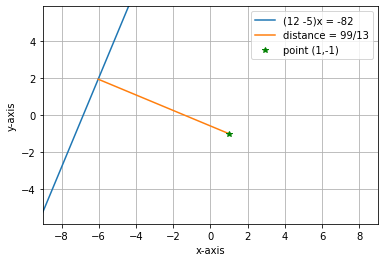
\includegraphics[width=\columnwidth]{./solutions/line_plane/33/output.png}
\caption{Plot showing the distance between the point and the line}
\label{fig:solutions/line_plane/33/}
\end{figure}
